\chapter{Discussão}

Nesta seção são analidos os resultados obtidos na seção anterior a fim de responder as perguntas que motivaram esse estudo.

\section{Algoritmos linear mais eficiente}

A primeira pergunta a ser respondida é qual dos dois algoritmos lineares simulados são mais eficientes. Na figura \ref{fig:lvsj_search_time}, estão os resultados da busca linear e da {\it jump search} da seção anterior. Claramente a {\it jump search} é mais rápida, chegando a ser mil vezes mais rápida para o maior tamanho de arranjo. Na ampliação mostrada na figura \ref{fig:lvsj_search_time_zoom} podemos observar melhor a diferença de eficiência entre os dois algoritmos. 

\begin{figure}[H]
  \centering
  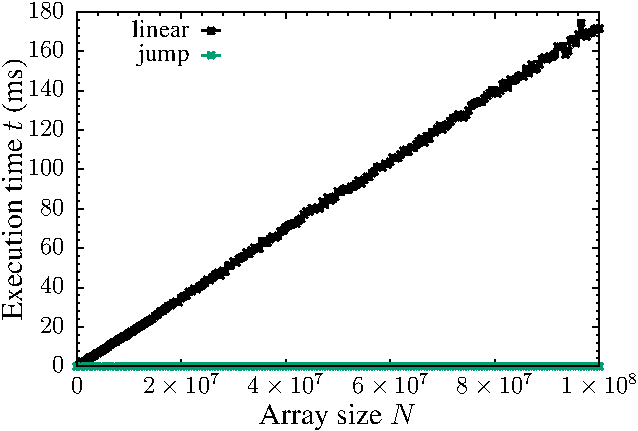
\includegraphics[scale=1.2]{../plots/lvsj_search_time.pdf}
 \caption{Comparação do tempo de execução médio das simuluções dos algoritmos lineares: busca linear (preto) e {\it jump search} (verde).}
\end{figure} \label{fig:lvsj_search_time}

\begin{figure}[H]
  \centering
  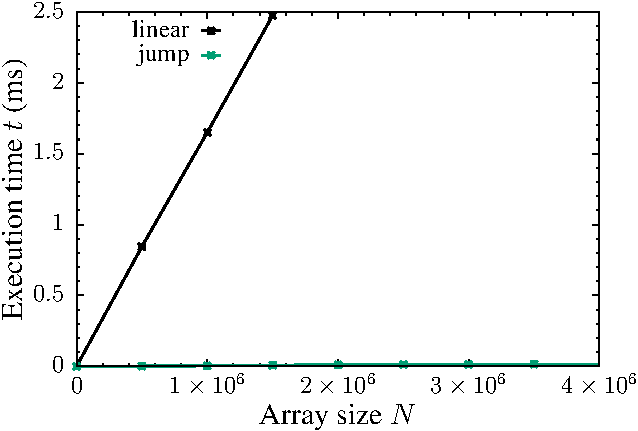
\includegraphics[scale=1.2]{../plots/lvsj_search_time_zoom.pdf}
  \caption{Ampliação da figura \ref{fig:lvsj_search_time}.}
\end{figure} \label{fig:lvsj_search_time_zoom}


\section{Implementação mais eficiente: recursiva ou iterativa?}

O segundo objetivo é determinar qual implementação é mais eficiente, a recursiva ou iterativa. Na figura \ref{fig:bsearch_ivsr_time}

\begin{figure}[H]
  \centering
  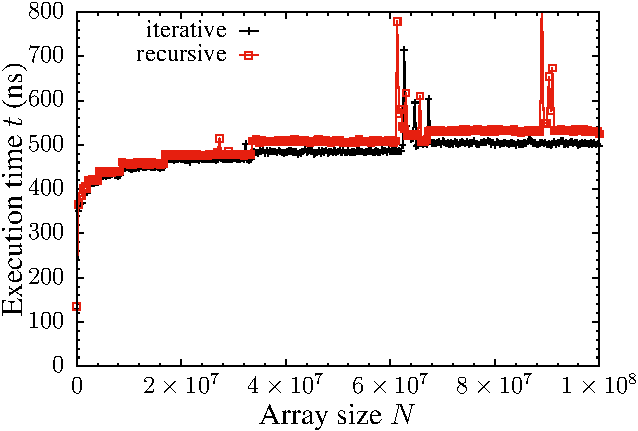
\includegraphics[scale=1.2]{../plots/bsearch_itvsrec_time.pdf}
  \caption{Comparação do tempo de execução médio das simuluções da implementação iterativa (preto) e recursiva (vermelho) do algoritmo de busca binária.}
\end{figure} \label{fig:bsearch_ivsr_time}

\begin{figure}[H]
  \centering
  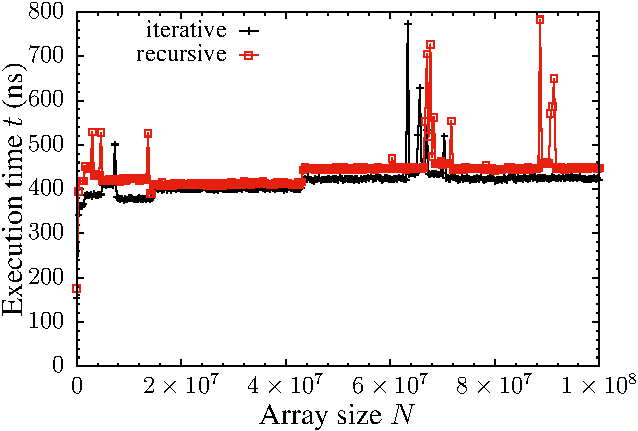
\includegraphics[scale=1.2]{../plots/tsearch_itvsrec_time.pdf}
  \caption{Comparação do tempo de execução médio das simuluções da implementação iterativa (preto) e recursiva (vermelho) do algoritmo de busca ternária.}
\end{figure} \label{fig:tsearch_ivsr_time}


\section{Influência do tamanho da partição nos algoritmos de busca não lineares}

O terceiro, é determinar como o tamanho da partição influência nos algoritmos de busca não lineares.

\begin{figure}[H]
  \centering
  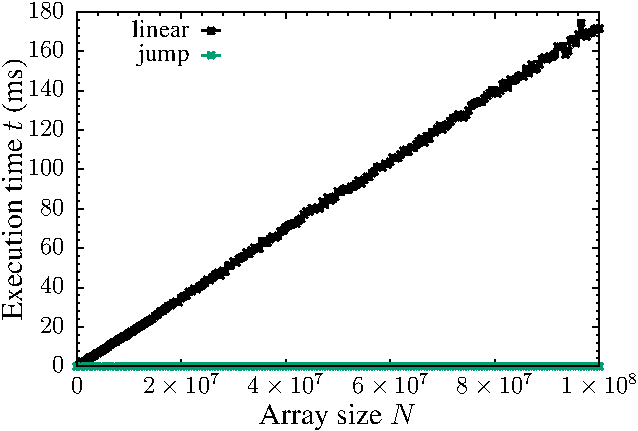
\includegraphics[scale=1.2]{../plots/lvsj_search_time.pdf}
%  \caption{Comportamento assintótico da {\it jump search} em relação ao tempo de execução médio (medido em milisegundos) a medida que o tamanho do arranjo sequencial $N$ aumenta.}
\end{figure} \label{fig:lvsj_search_time}


\section{Diferenciação de algoritmos de classe de complexidade diferentes}

O quarto é determinar a partir de que momento algoritmos de classe de complexidade diferentes se diferenciam, comparando a busca linear com a binária.

\begin{figure}[H]
  \centering
  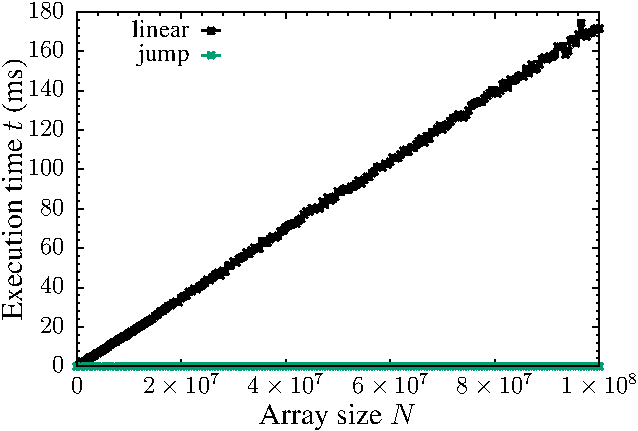
\includegraphics[scale=1.2]{../plots/lvsj_search_time.pdf}
%  \caption{Comportamento assintótico da {\it jump search} em relação ao tempo de execução médio (medido em milisegundos) a medida que o tamanho do arranjo sequencial $N$ aumenta.}
\end{figure} \label{fig:lvsj_search_time}

\section{Cenários do algoritmo de Fibonacci}

Por fim, o quinto objetivo procura determinar se existe diferentes categorias de cenários de pior caso para o algoritmo de busca de Fibonacci.

\begin{figure}[H]
  \centering
  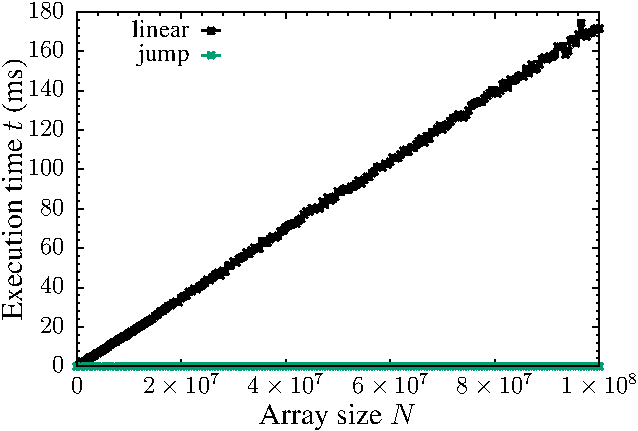
\includegraphics[scale=1.2]{../plots/lvsj_search_time.pdf}
%  \caption{Comportamento assintótico da {\it jump search} em relação ao tempo de execução médio (medido em milisegundos) a medida que o tamanho do arranjo sequencial $N$ aumenta.}
\end{figure} \label{fig:lvsj_search_time}
